% Figure block for the multimodal scaling subsection (fig_mm_scaling.pdf).
% v2 token-boundary cover-EM, 1500-q fixed eval, Qwen2.5-VL-7B reader over top-5, InfoSeek val,
% 422K-passage corpus. Whiskers = seed min--max where more than one seed exists.
%
% REPRO(fig:mm_scaling): regenerate from the result jsons -- the script hand-types NOTHING:
%   MMRAG_DATA=<data> python3 mmrag/plot_scaling.py --out mmrag/fig_mm_scaling
% It discovers runs by CONFIG EQUIVALENCE against a per-series reference run (a run joins a
% series iff its args.json differs from the reference only in seed / pool size / output paths),
% reads the recipe off args.json (v1 = algo grpo|ppo, v2 = plgrpo cc>0, v3 = plgrpo cc==0), and
% prints its own provenance block on every run. Pending cells are simply absent from the plot.
% Values at the commit that produced the current PDF:
%   zero-shot base   gme2b-zeroshot-3k-repro = 0.3080
%   relevance-SFT    sft-lr1e4-h0-repro      = 0.3100
%   v1 RECORDED wave 2k 0.3333 / 8k 0.3407 / 41k 0.3415 (4 seed replicates)
%   v1 FRESH wave    12.5k 0.3433 / 25k 0.3462 (3 seeds) / 50k 0.3467 / 100k 0.3287 / 200k 0.3480
%   v3 FRESH wave    45,248 (all of pool_train) 0.3471 (3 seeds)
% CAPTION HISTORY: the previous caption ("Multimodal indirect feedback SCALES; direct
% supervision does not", pushed at e5c3acc, recorded-wave era) predated the fresh ladder and
% was contradicted by the very cells this figure now shows. Do not restore it.
% CAUTION for whoever edits the script: on the recorded wave, axes-equivalence alone also admits
% the data-mix, frozen-index and 7B-reward cells (9 runs instead of 4) because results_summary
% has no field for those axes -- RECORDED_FAMILY exists to exclude them. On the fresh wave, the
% per-series `pools` allowlist exists to keep the scale-small* control out of the ladder.
\begin{figure}[t]
\centering
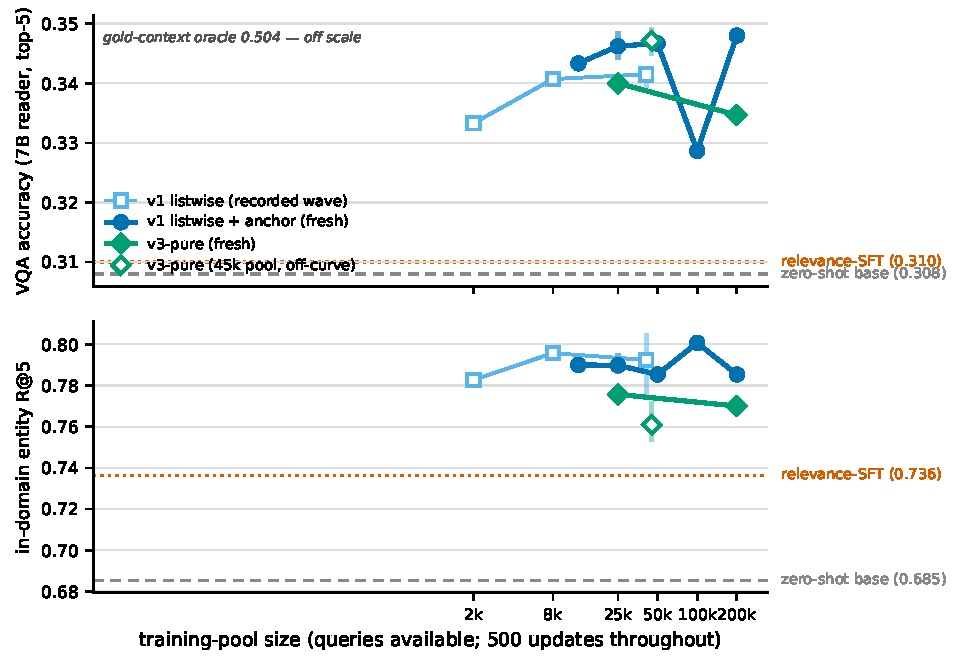
\includegraphics[width=0.72\textwidth]{fig_mm_scaling.pdf}
\caption{\textbf{The ceiling is a property of the recipe, not of the data budget.} Downstream
VQA accuracy of the frozen \textsc{Qwen2.5-VL-7B} reader (top-$5$) for \textsc{GME-Qwen2-VL-2B}
retrievers trained on nested InfoSeek query subsets at fixed compute ($500$ updates throughout).
Across a $16\times$ range of available training data the curve is flat to within $2$ points and
never approaches a data-limited regime, because at $500$ steps $\times$ batch $4$ only
${\sim}2{,}000$ queries are ever visited. \emph{Both ladder series are the v1 listwise recipe}
(anchored, deterministic top-$8$): filled circles are fresh same-cluster retrains, open squares
the pre-cluster-move recorded wave, shown separately because absolute levels are not comparable
across waves. The single \textsc{v3-pure} point is the headline three-seed cell at $45{,}248$
queries (all of \texttt{pool\_train}, a different and smaller pool file than the ladder's); the
matching v3 scaling cells are in flight, so \textbf{the data-scaling behaviour of the corrected
policy gradient is not yet measured} and no v3 curve should be read into this figure. Dashed
lines are the fresh zero-shot and relevance-SFT reproductions. Whiskers: seed min--max.}
\label{fig:mm_scaling}
\end{figure}
